\documentclass[british]{beamer}

\usepackage{default}
\usepackage[british]{babel}
\usepackage{epstopdf}
\usetheme{Madrid}
\usepackage{graphicx}
\usepackage{dirtytalk}
\usepackage{csquotes}


\begin{document}
%
\title[TIS Project]
{Document Semantic Similarity}

\subtitle{TIS Project}

\author[A. Pirovano, F. Picciotti]
{Alberto Pirovano \and Francesco Picciotti}

\institute[PoliMi]
{
	Politecnico di Milano
}

\logo{
	
\includegraphics[height=1.7cm,trim={0 2cm 4.5cm 2cm},clip]
	{./Imgs/Politecnico-di-Milano-3-m8qw.eps}
	}	

\AtBeginSection[]
{
	\begin{frame}
		\frametitle{Outline}
		\tableofcontents[currentsection]
	\end{frame}
}

\maketitle

\section{State of art}

	\begin{frame}{Introduzione}
		L'attuale stato dell'arte per similitudine semantica tra documenti si suddivide in:
		\begin{itemize}
			\item NLP Tradizionale \pause 
			\item Geometrico \pause
			\item Deep Learning based \pause 
		\end{itemize}
	\end{frame}
	
	\begin{frame}{NLP Tradizionale}
		Questo approccio segue la letteratura del Natural Language Processing e consiste dei seguenti passi:
		\begin{itemize}
			\item Cleaning dei dati
			\item Pos-Tagging
			\item Stemming o Lemmatisation
			\item Parsing
			\item Ontologia
		\end{itemize}
		Tuttavia nel caso del nostro scopo presenta delle criticit\`{a}, ovvero:
		\begin{itemize}
			\item Affidabilit\`{a} del Pos-Tagger italiano di TreeTagger
			\item Reperire una Ontologia e un parsing toll nella lingua italiana
		\end{itemize}\pause
	\end{frame}
	
	\begin{frame}{Geometrico}	
		\`{E} basato sulla rappresentazione vettoriale del documento, dove le diverse dimensioni sono il Bag of Word di tutti i documenti.
		Questo approccio richiede dei seguenti steps:
		\begin{itemize}
			\item Cleaning dei dati
			\item Stemming o Lemmatisation
			\item Encoding del documento in vettore
			\item TF/IDF + LSA (Latent semantic analysis)
		\end{itemize}
	\end{frame}
	
	\begin{frame}{...limiti?}
			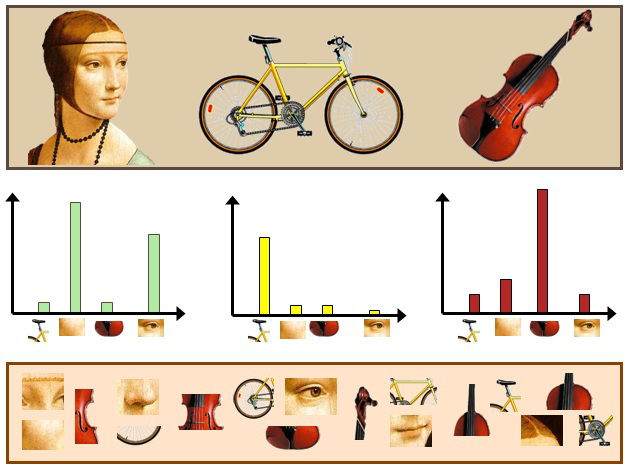
\includegraphics[width=0.9\textwidth, height=0.8\textheight]{./Imgs/bow-example.jpeg}
	\end{frame}
	
	\begin{frame}{Geometrico: limiti}
		Per riassumere:
		\begin{itemize}
			\item Molto dipendente dal preprocessing del corpus
			\item Grande Bag Of World $\rightarrow$ bisogno di LSA, ma non \`{e} così banale. 
			
			Perch\'{e}?
			\begin{displayquote}
				"LSA assumes that words that are close in meaning will occur in similar pieces of text"
			\end{displayquote}
			\item Un documento \`{e} un insieme \alert{non ordinato} di parole  
		\end{itemize}	
	\end{frame}
	
	\begin{frame}{Deep Learning}
		Negli ultimi anni il Deep Learning trova numerose applicazioni con ottimi risultati.\par
		La creazione di Word2Vec da Google offre un modello che ha principalmente, i seguenti vantaggi e svantaggi.
		\begin{columns}
			\column{0.5\textwidth}
			\underline{Pros:}
			\begin{itemize}
				\item Molto meno dipente da un preprocessing
				\item Context-aware
				\item Combina il metodo \textit{Geometrico} con quello \textit{NLP Tradizionale}
				\item Non sfrutta una ontologia, ma la \alert{crea} 
			\end{itemize}
			\column{0.5\textwidth}
			\underline{Cons:}
			\begin{itemize}
				\item Tecnica unsupervised 
				\item Bisogno di un esperto per validare gradi di similarità
				\item Pu\`{o} risultare in GIGO system (Garbage In Garbage Out)
			\end{itemize}
		\end{columns}
	\end{frame}
	
\section{Preprocessing}

\begin{frame}{Ciaone}
	\begin{displayquote}
		"Preprocessing is 80\% of NLP work"
		 
		\begin{flushright}
			\textit{Lev Konstantinovskiy}
		\end{flushright}
	\end{displayquote}
		
	Qui spieghiamo il preprocessing e visualizzazione (volendo)
\end{frame}

\section{Word2Vec}

\begin{frame}{Hello}
	Qui speghiamo per bene come funziona word2vec
\end{frame}

\section{Doc2Vec}


\begin{frame}{Hello}
	Qui speghiamo per bene come funziona word2vec\end{frame}
\end{document}
